\section{Visual Studio 2022}
\author{Mirzet sakonjic}
\subsection*{Erklärung}
Visual Studio Enterprise 2022 ist eine integrierte Entwicklungsumgebung für verschiedene Hochsprachen von Microsoft welche im Jahr 2022 (Juni) veröffentlicht wurde.
Visual Studio ermöglicht es Programmierern, sowohl Win32/Win64-Programme als
auch Anwendungen für das .NET Framework zu entwickeln. Darüber hinaus lassen sich
mit Visual Studio Windows-Apps, dynamische Webseiten bzw. Webservices für das
Internet/Intranet oder Azure-Services entwickeln.
\subsection*{Funktionalität}
Visual Studio ist eine sehr umfangreiche und komfortable Entwicklungsumgebung. Sie
lässt sich gezielt auf die Anforderungen von Projekten anpassen. Mit dem VS-Installer
können zusätzliche Hochsprachen installiert oder deinstalliert werden.
Neben der Erweiterbarkeit stellt Visual Studio einen integrierten Debugger zur Verfügung. Dieser enthält die Funktion „Bearbeiten und Fortfahren“ und erlaubt das
nachträgliche Anhängen an bereits laufende Prozesse, sowohl am lokalen Rechner als
auch über das Netzwerk. Neben dem Debugger wird der Softwareentwickler durch eine
gute IntelliSense unterstützt.
\subsection*{Begründung und Verwendung}
Visual Studio ist die etablierteste Entwicklungsumgebung auf dem Markt, um .NET
zu programmieren, da es sich durch seinen Umfang und die gute Bedienbarkeit ausgezeichnet. Aufgrund der vielen Funktion, der Marktposition und der Tatsache, dass
sich Visual Studio bereits in vergangenen Projekten bewährt hat, wurde es für unsere
Arbeit gewählt. Die Enterprise Lizenz wurde von der HTL zur Verfügung gestellt und
darf ausschließlich für schulische Zwecke eingesetzt werden.


\section{Visual Studio Code}
\author{Stefano Pyringer}

% Bilder sollten nebeneinander sein
\begin{figure}[htb]
    \begin{center}
        
\includegraphics[width=3cm] {./pics/Visual_Studio_Code_1.35_icon.svg.png}
        \caption{Visual Studio Code Logo}
        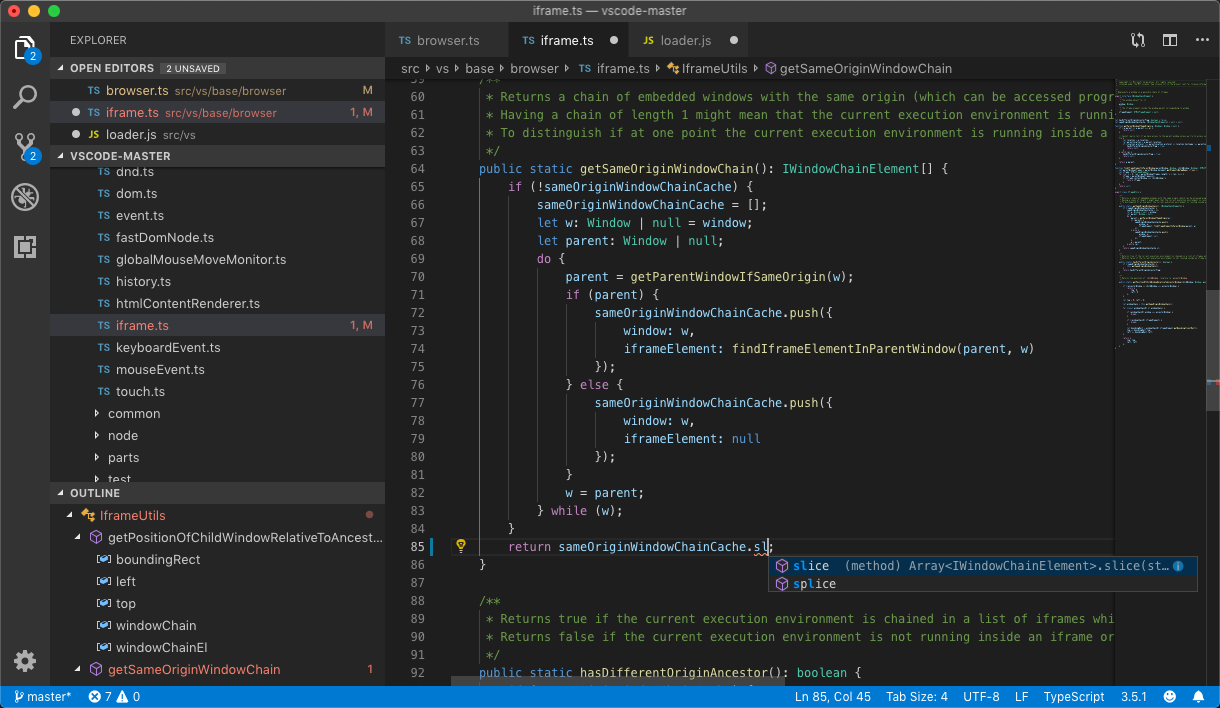
\includegraphics[width=6cm]{./pics/VS_Code_1.36.0-insider.png}
        \caption{Visual Studio Code Screenshot}
    \end{center}
\end{figure}

Visual Studio Code, wird auch als VS Code bezeichnet, ist ein Code-Editor entwickelt von Microsoft. 
Seit November 2015 ist der Source-Code des Code-Editors auf Github verfügbar. Im April 2016 wurde die erste finale Version 
von Visual Studio Code veröffentlicht. Der Source-Code von des Code-Editors mit einer MIT-Lizenz lizensiert und ist somit Open-Source.
Das installierbare Programm hingegen enthält Microsoft-Binaries und ist deshalb keine Open-Source. Das Programm ist kostenlos verfügbar.

Der Texteditor basiert auf dem App-Framework Electron und läuft daher in der Chromium-Engine. Standardmäßig werden ohne zusätzliche Instalationen
die gängigen Programmier- und Scriptsprachen wie HTML, JavaScript, SQL, JSON, C und viele weitere unterstützt. 
Folgende Basisfunktionen besitzt das Entwickler-Tool:

\begin{itemize}
    \item Syntaxhervorhebung
    \item Autovervollständigung
    \item Code-Folding (ev. Erklärung Fusszeile!)
    \item Debugging
    \item Versionsverwaltung
    \item Konfigurierbare Code-Snippets
    \item IntelliSense für TypeScript, JSON, CSS und HTML
    \item Extension-Support
\end{itemize}

\subsection{Unterschiede zu Visual Studio}
Entwicklungsumgebungen (IDEs) wie Visual Studio sind meistens für ein Betriebssystem entwickelt worden und funktionieren 
gar nicht oder nur eingeschränkt auf anderen Betriebssystemen. Die Auswahl von Programmiersprachen und Frameworks ist beschränkt. IDEs 
haben üblicherweise einen hohen Speicher- und Ressourcenbedarf.

Visual Studio Code hingegen ist ein Texteditor, der in der Chromium-Engine läuft und ist für alle 3 gängigen Betriebssysteme 
Windows, MacOs und Linux verfügbar. Aufgrund des niedrigen Ressourcenbedarfs ist es auch auf schwächeren oder älteren Computern und Laptops benutzbar.
Ein großer Unterschied zu Visual Studio ist die Dateiveraltung. 
In Entwicklungsumgebungen wird ein Projekt in Projektdateien zusammengefasst, 
währendessen der Code-Editor mit Workspaces arbeitet. Diese speichern den 
Bearbeitungszustand, Reihenfolge und Zeilenposition der geöffneten Dateien. 
In Visual Studio Code wird ein Workspace geöffnet, indem ein Ordner ausgewählt wird.

Ein Texteditor kann den Funktionsumfang und Komfort einer Entwicklungsumgebung nicht mithalten. Visual Studio Code 
kann dank Plug-ins, werden auch als Extensions bezeichnet, in der Funktionalität stark erweitert werden.
Ein großer Vorteil zu Visual Studio ist der Extension-Marketplace, die von einer großen Gemeinschaft von Entwicklern gepflegt wird.
Dank einer Vielzahl von Plug-ins ist fast jede beliebige Sprache verfügbar mit umfangreichen Hilfsfunktionen wie IntelliSense oder Snippets verfügbar.

\subsection{Thunder Client Extension}
\author{Stefano Pyringer}


\subsection{ERD Editor Extension}
\author{Stefano Pyringer}


\section{Github}
\author{Mirzet Sakonjic}
\subsection*{Erklärung}
GitHub ist ein webbasiertes Unternehmen zur Versionsverwaltung von Software - Entwicklungsprojekten. Dies bedeutet, dass man mit mehreren Entwicklern zusammenarbeiten kann. GitHub
gibt es seit 2007. Es ist egal, welche Programmiersprache angewendet wird. Es ist
deshalb auch vorteilhaft, weil man die Software versionieren und dadurch, wenn sich
ein Fehler eingeschlichen hat zu einer früheren Version zurückkehren kann.
\subsection*{Funktionalität}
Damit man an einem Programm, einer Website oder Ähnlichem mitarbeiten bzw. diese
ansehen kann, muss das Repository, also das Verzeichnis, öffentlich sein bzw. muss man
dazu eingeladen werden, ist dies nicht der Fall, kann nur der Ersteller des Reposiotrys
daran arbeiten.
Dabei können beliebig viele Entwickler an einem Verzeichnis arbeiten. Damit man
mitarbeiten kann, muss man das Repository forken, was bedeutet eine Kopie in seinem
eigenen Konto mit den derzeitigen Daten zu erstellen.
Später können, wenn der Ersteller des ursprünglichen Reposiotry es zulässt, die zwei
Repositorys wieder zusammengeführt werden. Dies heißt mergen. Man kann auch einem
Repository oder Entwickler nur folgen. GitHub wird von Microsoft betreut.
\subsection*{Begründung und Verwendung}
Es wurde verwendet, da es der einfachste zu bedienende Dienst zum Verwalten von
Versionen eines Programms oder einer Website ist. Es wurde für FrontEnd, BackEnd
und Dokumentation verwendet.

\section{Testen auf dem Endgerät}
\subsection{Android Emulator}
\subsection{iOS Emulator}